%% LyX 2.3.2 created this file.  For more info, see http://www.lyx.org/.
%% Do not edit unless you really know what you are doing.
\documentclass[english]{article}
\usepackage{lmodern}
\usepackage[T1]{fontenc}
\usepackage[latin9]{inputenc}
\usepackage{geometry}
\geometry{verbose,tmargin=2cm,bmargin=2.5cm,lmargin=2.3cm,rmargin=2cm}
\usepackage{verbatim}
\usepackage{float}
\usepackage{graphicx}

\makeatletter
%%%%%%%%%%%%%%%%%%%%%%%%%%%%%% Textclass specific LaTeX commands.
\newcommand{\lyxaddress}[1]{
	\par {\raggedright #1
	\vspace{1.4em}
	\noindent\par}
}

%%%%%%%%%%%%%%%%%%%%%%%%%%%%%% User specified LaTeX commands.
\usepackage{lipsum}
\usepackage{xr}
\externaldocument{Paper_req-550_V0.4_SM}
\usepackage{lineno}
\usepackage[strings]{underscore}

\makeatother

\usepackage{babel}
\begin{document}
\title{Empowering the crowd: Feasible strategies \\ to minimize the spread
of COVID-19 \\ in high-density informal settlements}
\author{Alberto Pascual-Garc�a$^{(1,*)}$, Jordan Klein$^{(2)}$, Jennifer
Villers$^{(2,\land)}$, \\ Eduard Campillo-Funollet$^{(3,\wedge)}$,
Chamsy Sarkis$^{(4)}$}

\maketitle
\medskip{}


\lyxaddress{\begin{center}
(1) Institute of Integrative Biology. ETH-Z�rich. Z�rich, Switzerland
\\ (2) Woodrow Wilson School. Princeton University. Princeton, NJ,
USA. \\ (3) Genome Damage and Stability Centre, University of Sussex,
Brighton, United Kingdom \\ (4) Pax Syriana Foundation, Valetta,
Malta \\ ($\land$) Equal contribution. \\ ({*}) correspondence:
alberto.pascual@env.ethz.ch
\par\end{center}}

\newpage{}
\begin{abstract}
\textbf{\normalsize{}Background\medskip{}
}{\normalsize\par}

{\normalsize{}More than 1 billion people live in informal settlements
worldwide, in which the established paradigm to contain the spread
of COVID-19 through social distancing, hygiene measures, and generalized
use of personal protection equipment, present additional challenges.
We investigated the impact of adapting these measures to informal
settlements located in regions immerse in procrasted conflicts, which
should additionally contend with the public health challenges resulting
from violence, the deterioration of health-systems, and the political
unstability which precludes coordinated action.}{\normalsize\par}

\textbf{\normalsize{}\medskip{}
}{\normalsize\par}

\textbf{\normalsize{}Methods}{\normalsize\par}

\textbf{\normalsize{}\medskip{}
}{\normalsize\par}

{\normalsize{}We implemented a stochastic Susceptible-Exposed--Infectious-Recovered
model to simulate the spread of the virus in high-density camps of
Internally Displaced Persons, with a population structure representative
of the Northwest region of Syria. We chose parameters corresponding
to a worst-case scenario in which no health-system is available. We
evaluated interventions adapted to the living conditions in the camps,
including self-distancing, self-isolation and the protection of vulnerable
population in safety zones. We considered details representating social
and technical challenges, which influence the micro-dynamics of the
model.}{\normalsize\par}

\textbf{\normalsize{}\medskip{}
}{\normalsize\par}

\textbf{\normalsize{}Findings}{\normalsize\par}

\textbf{\normalsize{}\medskip{}
}{\normalsize\par}

{\normalsize{}All the interventions have a significant effect in reducing
the probability of observing a global outbreak in the camp and the
death tolls. Self-distancing brings the best results overall, if a
50\% reduction in the number of contacts was considered, with mortality
reduced up to a 35\%. }%
\begin{comment}
However, this reduction is close to the maximum we estimate as realistic,
and the fraction of the population recovered is lower than with other
interventions
\end{comment}
{\normalsize{}. A similar reduction in the casualties is achieved
making available 1 tent for self-isolation per 200 individuals. Protecting
vulnerable population in a safe area of the camp have synergistic
effects with previous interventions for the whole population, and
it is particularly beneficial for the vulnerable population. Complementaary
mesaures such as the lockdown of the safety zone, further reduce the
probability of an outbreak and the number of casualties. Importantly,
the time at which the number of symptomatic individuals will peak
is delayed with most of the interventions, in some cases by more than
three months, and the proportion of the population recovered, near
a 70\%, could be compatible with herd immunity. The combination of
interventions may reduce the mortality as much as 80\%.}{\normalsize\par}

\textbf{\normalsize{}\medskip{}
}{\normalsize\par}

\textbf{\normalsize{}Interpretation}{\normalsize\par}

\textbf{\normalsize{}\medskip{}
}{\normalsize\par}

{\normalsize{}Our results highlight the potential of non-medical interventions
to mitigate the effects of the epidemic. We demonstrate that interventions
that were proved effective in other settings could be adapted to the
camps. When the parameters considered have values that could be considered
inefficient implementations of the interventions we still observed
beneficial effects for the individual interventions and for their
combination. The quantification we provide for specific details influencing
the interventions such as the existence of buffer zones, daily health-checks,
or the number of carers per isolated individual, suggest that the
interventions are feasible and highlight the best avenues to implement
them. The low cost and rapid applicability of the interventions support
their idoneity, whose implementation would hence become mostly limited
by the acquisition of local-communities of the necessary knowledge
and means to incorporate them.}{\normalsize\par}

\textbf{\medskip{}
}

\begin{comment}
Funding
\end{comment}

\newpage{}
\end{abstract}

\part*{Introduction}

The COVID-19 pandemic is intensifying in the developing world \cite{Guardian1M}.
In Africa, SARS-CoV-2 has been spreading from urban areas to informal
settlements \cite{WHO_AfricaMarks6months}. With more than 1 billion
people living in informal settlements worldwide, urgent action is
needed to contain the virus in these settings, a task which necessarily
involves the engagement of the communities living in them \cite{wilkinson_local_2020}.

The need for action is even more pressing in regions immersed in protracted
armed conflicts, where large portions of their populations have become
displaced. When the displaced population exceeds official resettlement
and refugee camp capacity, Internally Displaced Persons (IDPs) must
live in informal settlements (hereafter named ``camps''). These
regions must contend with the public health challenges resulting from
violence \cite{abbas_migrant_2018}, the deterioration of health-systems
\cite{hill_conflict_2010}, especially of critical care \cite{sahloul_war_2016},
and the breakdown of essential public infrastructure such as water
and sanitation systems \cite{sikder_water_2018}.

This study focuses on the Northwest region of Syria (NWS): a relatively
small geographical area with 4.2 million people, of which 1.15 million
(27.4\%) are IDPs living in camps \cite{Health_directorate}. The
health status of households in camps in NWS is poor; 24\% have a member
with a chronic disease, of whom 41\% have no access to medicines \cite{noauthor_syria_nodate}.
As in other conflict regions, the political instability in NWS hinders
coordinated public health actions, and the ongoing movements of IDPs
create ample opportunity for infectious disease transmission, while
making contact tracing interventions infeasible.

To investigate feasible COVID-19 prevention interventions in the camps,
we considered a Susceptible-Exposed-Infectious-Recovered model in
which the camps' populations are divided into classes reflecting their
estimated age-structures and comorbidity prevalence. We use this model
to propose various interventions aimed at reducing the number of contacts
within and between population classes in general, and with symptomatic
individuals in particular. We paid special attention to how the living
conditions in informal camps inform the assumptions underlying our
proposed interventions. We modeled interventions previously proposed
for African cities \cite{vanzandvoort2020}, such as self-distancing,
isolation of symptomatic individuals and the creation of a 'safety
zone' in which more vulnerable members of the population are protected
from exposure to the virus.

Building upon the approach used to model the impact of these interventions
in African cities, our model includes a parameterization of the contacts
each individual has per day \cite{vanzandvoort2020}. We further elaborate
upon this approach by making a more explicit representation of contacts
and other parameters in the model. We consider the micro-dynamics
of contacts, the time that individuals take to recognize their symptoms
before self-isolating, the effect of having carers to attend to isolated
individuals, and the existence of a buffer zone in which exposed and
protected population classes can interact under certain rules. We
examine a potential worst-case scenario in which there is no access
to any healthcare facility. Since empowering local communities in
conflict regions to understand how to control COVID-19 is possibly
the most (and perhaps only) effective way to minimize its spread,
our models are of utmost importance for informing the implementation
of realistic interventions in these regions.

\part*{Methods}

\subsection*{The model}

We considered a discrete-time stochastic model, simulating a viral
outbreak in a single camp over a 12 month period. The model is divided
into compartments containing individuals at different possible stages
along the disease's progression (see Supplementary Fig. \ref{fig:Diagram}),
and splits the population into classes by age and comorbidity status.
The simulation starts with a completely susceptible population where
one person is exposed to the virus. The disease in exposed individuals
progresses through a preclinical infectious stage, followed by either
a clinical (symptomatic) or subclinical (asymptomatic) infectious
stage, resolving through recovery or death. Additional susceptible
individuals become infected through contact with infectious individuals.
We verified that a steady state was always reached before the end
of each simulation. We did not consider migration, births, nor deaths
due to other causes, since they are small enough in magnitude to not
significantly impact the course of an outbreak, provided additional
conflict does not erupt.

\subsection*{Population structure}

We parameterized the model with data from IDPs in NWS \cite{noauthor_syrian_nodate}.
The population size of informal camps approximately log-normal, with
a mean of 940 individuals. We simulated camps with 500, 1000 and 2000
individuals. Since interventions tend to be less effective in larger
camps, the results presented refer to simulations with 2000 individuals,
unless otherwise specified. We considered 3 age groups: children (age
1, 0-12 years old), working-age adults (age 2, 13-50 yrs.) and older
adults (age 3, >50 yrs). For ages 2 and 3, we considered two subclasses
comprising healthy individuals and individuals with comorbidities.
The fraction of a simulated camp's population in each of these 5 classes
is shown in Supplementary Table \ref{tab:PopParams}%
\begin{comment}
Alberto insert SM cross-ref
\end{comment}
.

\subsection*{Epidemiological severity assumptions}

In NWS, there are 4 active and 2 in plan COVID-19 referral hospitals
with 66 ventilators and current capacity of 74 ICU beds and 355 ward
beds,  for 4.2 million people \cite{REACH_syriaOverview,UNOCHA_health_numbers}.
Basic estimation predicted a collapse of the health facilities after
8 weeks of the outbreak \cite{hariri_SyriaForecast_2020}. Hence,
we considered a worst-case scenario in which individuals will not
have access to healthcare. We consequently assumed that all critical
cases, those requiring ICU care, would die. However, there is greater
uncertainty about the fate of severe cases, those requiring hospitalization
but not ICU care. We therefore considered a compartment for severe
cases to account for a longer infectious period if they stay in the
camp. This compartment also helped us model some interventions more
realistically, for example by noting that the symptoms of severe cases
are incompatible with self-isolation. To estimate upper and lower
bounds for the outcome variables of our model, we simulated two possible
scenarios for the fate of this compartment: one in which all cases
recover, and another in which all die. In the simulations presented
in the Main Text, we consider the worst-case scenario in which all
of these cases die.

The fractions of symptomatic cases that are severe or critical are
class-specific (parameters $h_{i}$ and $g_{i}$, see Supplementary
Table \ref{tab:PopParams}). We estimated these parameters using data
from developed countries with superior population health \cite{dong2020epidemiological,covid2020preliminary}.
Following previous work \cite{vanzandvoort2020}, we reasoned that
the case severity distributions of NW Syrian adult population classes
would correspond with those of older age groups in developed countries.

\subsection*{Transmissibility assumptions}

We assumed presymptomatic, asymptomatic, symptomatic and hospitalized
individuals were equally infectious. We obtained the duration individuals
spend in each compartment from the literature (see Supplementary Table
\ref{tab:FixedParams}). Each individual's contact rate (see Supplementary
Table \ref{tab:PopParams}) is class-specific, and was estimated from
conversations with camp managers in NWS. The probability of random
interaction with an individual from each class is proportional to
this class' fraction of the population. The product of these two values
is the contact rate between two respective classes.

The probability of infection from contact with an infectious individual,
$\tau$, was estimated from a Gaussian distribution of the basic reproduction
number, $R_{0}$, with a mean of 4 (99\% CI: 3--5). This distribution
was a compromise between values reported in the literature from regions
with high-density informal settlements: $R_{0}$=2.77 in Abuja and
3.44 in Lagos, Nigeria \cite{oyinlola_empirical_2020}, 3.3 in Buenos
Aires \cite{santos_numerical_2020}, and 5 in Rohingya refugee camps
in Bangladesh \cite{truelove_potential_2020}. The probability distribution
of $\tau$ was estimated by randomly generating a value for $R_{0}$,
and dividing this value by the real part of the main eigenvalue of
the Next Generation Matrix (see Supplementary Material).

\subsection*{Interventions}

\begin{figure}[H]
\includegraphics[width=1\textwidth]{figures/diagram_interventions}

\caption{\textbf{\label{fig:Interventions}Diagram of interventions.}}
\end{figure}


\subsubsection*{Self-distancing}

We considered a situation in which the whole population reduces their
mean number of contacts per day by a certain magnitude, 20\% or 50\%
(see Fig. \ref{fig:Interventions}-1). Since the mean number of people
per tent in a camp is 5.5 and sanitation facilities are shared \cite{noauthor_syrian_nodate}
we inferred that the number of contacts per day cannot be reduced
by more than 50\%. For an adult, this would mean 7.5 contacts per
day.

\subsubsection*{Buffer zone}

Since only moderate self-distancing can be achieved, additional control
measures involve splitting the population into subgroups occupying
different zones of the camp, limiting cross-group contacts to specified
locations, or ``buffer zones''. We envision these zones as open
spaces, with guidelines in place to limit occupancy to 4 individuals
wearing masks, with 2 meters separating individuals from the two separate
zones. Based on discussions with local organizations, we assumed a
level of non-compliance such that the probability of transmission
from contacts in these buffer zones will be reduced by 80\%, rather
than 100\%, compared to the baseline (see Fig. \ref{fig:Interventions}).

\subsubsection*{Self-isolation}

Self-isolation is a challenge in informal settlements, where households
consist of a single (often small) space, water is collected at designated
locations, sanitation facilities are communal and food supplies are
scarce. We considered the possibility of those showing symptoms self-isolating
in individual tents in dedicated parts of the camps, or next to the
tents of their relatives. We simulated this intervention with various
numbers of isolation tents per camp, ranging from 10 to 2000 for a
camp of 2000 people (see Fig. \ref{fig:Interventions}-2). In addition,
we modeled the role of carers dedicated to supplying isolated individuals,
who interact with them via a buffer zone (see Fig. \ref{fig:Interventions}-2a).
In considering one carer per individual with one contact per day,
we do not neglect their probability of infecting the rest of the camp.
We further considered that severe cases, or those in the hospitalized
compartment, are fully infectious since they require more intensive
care that is not possible to deliver while adhering to the guidelines
of the buffer zone. We also considered minimum time intervals for
individuals to recognize their symptoms: with means of 12, 24 and
48 hours (see Fig. \ref{fig:Interventions}-2b).Safety zone

In this intervention, the camp is divided in two areas: a safety zone,
in which more vulnerable people live (hereby referred to as a ``green''
zone following previous studies \cite{vanzandvoort2020}), and an
exposed (``orange'') zone with the remaining population. In our
simulations, the first exposed individual always belongs to the orange
zone. We avoided the use of the term ``shielding'' to describe this
intervention, since it may erroneously suggest that the vulnerable
population is isolated in a closed space, such as a separated building.
Such an intervention would require additional assumptions on how contacts
occur in closed spaces. The living conditions within both zones remain
the same, so the overall contact rate does not change unless self-distancing
is also implemented. In practice, reducing the contact rate with individuals
living in a different zone implies an increase in the contact rate
with individuals in the same zone (see Supplementary Material). This
allows us to investigate undesired side-effects of this intervention.
Since proposals for partitioning the population may be received differently
across camps, we considered several scenarios for allocating a camp's
population to the two zones (see Fig. \ref{fig:Interventions}-3,
Supplementary Table \ref{tab:SafetyScenarios}). We consider the scenario
in which all older adults, working-age adults with comorbidities and
their family members up to 20\% of the camp's population live in the
green zone in the Main Text, unless otherwise specified.

Interaction between the two zones is limited to a buffer zone. Individuals
in the green zone cannot leave and thus need to be provided with supplies
by individuals in the orange zone. Delivery of supplies will take
place in the buffer zone. In our simulations, we considered limiting
individuals in the green zone to 10 or 2 contacts with individuals
from the orange zone per week (see Fig. \ref{fig:Interventions}-3a).
Other variations of this intervention we explored include preventing
symptomatic individuals from entering the buffer zone (see Fig. \ref{fig:Interventions}-3b)
and a ``lockdown'' of the green zone, where the number of weekly
contacts in the buffer zone is reduced by 50\% or 90\% (see Fig. \ref{fig:Interventions}-3c).

\subsubsection*{Evacuation}

The last intervention we simulated is the evacuation of individuals
in the hospitalization compartment. We assume the evacuees will be
taken to isolation centers, not hospitals, so this measure does not
change their fate; the only effect this intervention has is reducing
the infectivity of evacuees to zero (see Fig. \ref{fig:Interventions}-4).

\subsection*{Analysis of the interventions}

For each implementation of the interventions, we ran 500 simulations
and compared results between them. The main variables considered are
the fraction of simulations in which at least one death is observed,
a proxy for the probability of an outbreak, the fraction of the population
that dies and the time until the symptomatic population peaks, as
well as the case fatality rate (CFR) and fraction of the population
that recovers. For consistency, we only considered simulations in
which there was an outbreak when comparing the outcome of a variable
between interventions. We used the Shapiro-Wilk test \cite{shapiro_analysis_1965}
to verify that our results do not exhibit normally distributed residuals,
Kruskal-Wallis test for pairwise comparisons \cite{kruskal_ranks_1952},
and Conover-Iman test for multiple comparisons \cite{conover_multiple_1979}.
The model and all statistical analysis were implemented in R \cite{R_2020};
we used the package PMCMRplus \cite{pohlert_pmcmr_2020}. All the
code and results are freely available at the url: https://github.com/crowdfightcovid19/req-550-Syria.

\subsection*{Role of the funding source}

The funders of the study had no role in study design, data collection,
data analysis, data interpretation, or writing of the article.

\part*{Results}

Without any interventions, the mean CFR is \textasciitilde 2\% in
simulations where all severe cases requiring hospitalization recover
(see Supplementary Fig. \ref{fig:Suppl_DvsR}), and \textasciitilde 11\%
in simulations where all severe cases die. We consider the latter
scenario to evaluate the interventions. In this scenario, the probability
of observing an outbreak is close to 0.85, in which \textasciitilde 10\%
of the camp dies, the number of symptomatic cases peaks after 55 days
and \textasciitilde 84\% of the population recovers.

\begin{figure}[H]
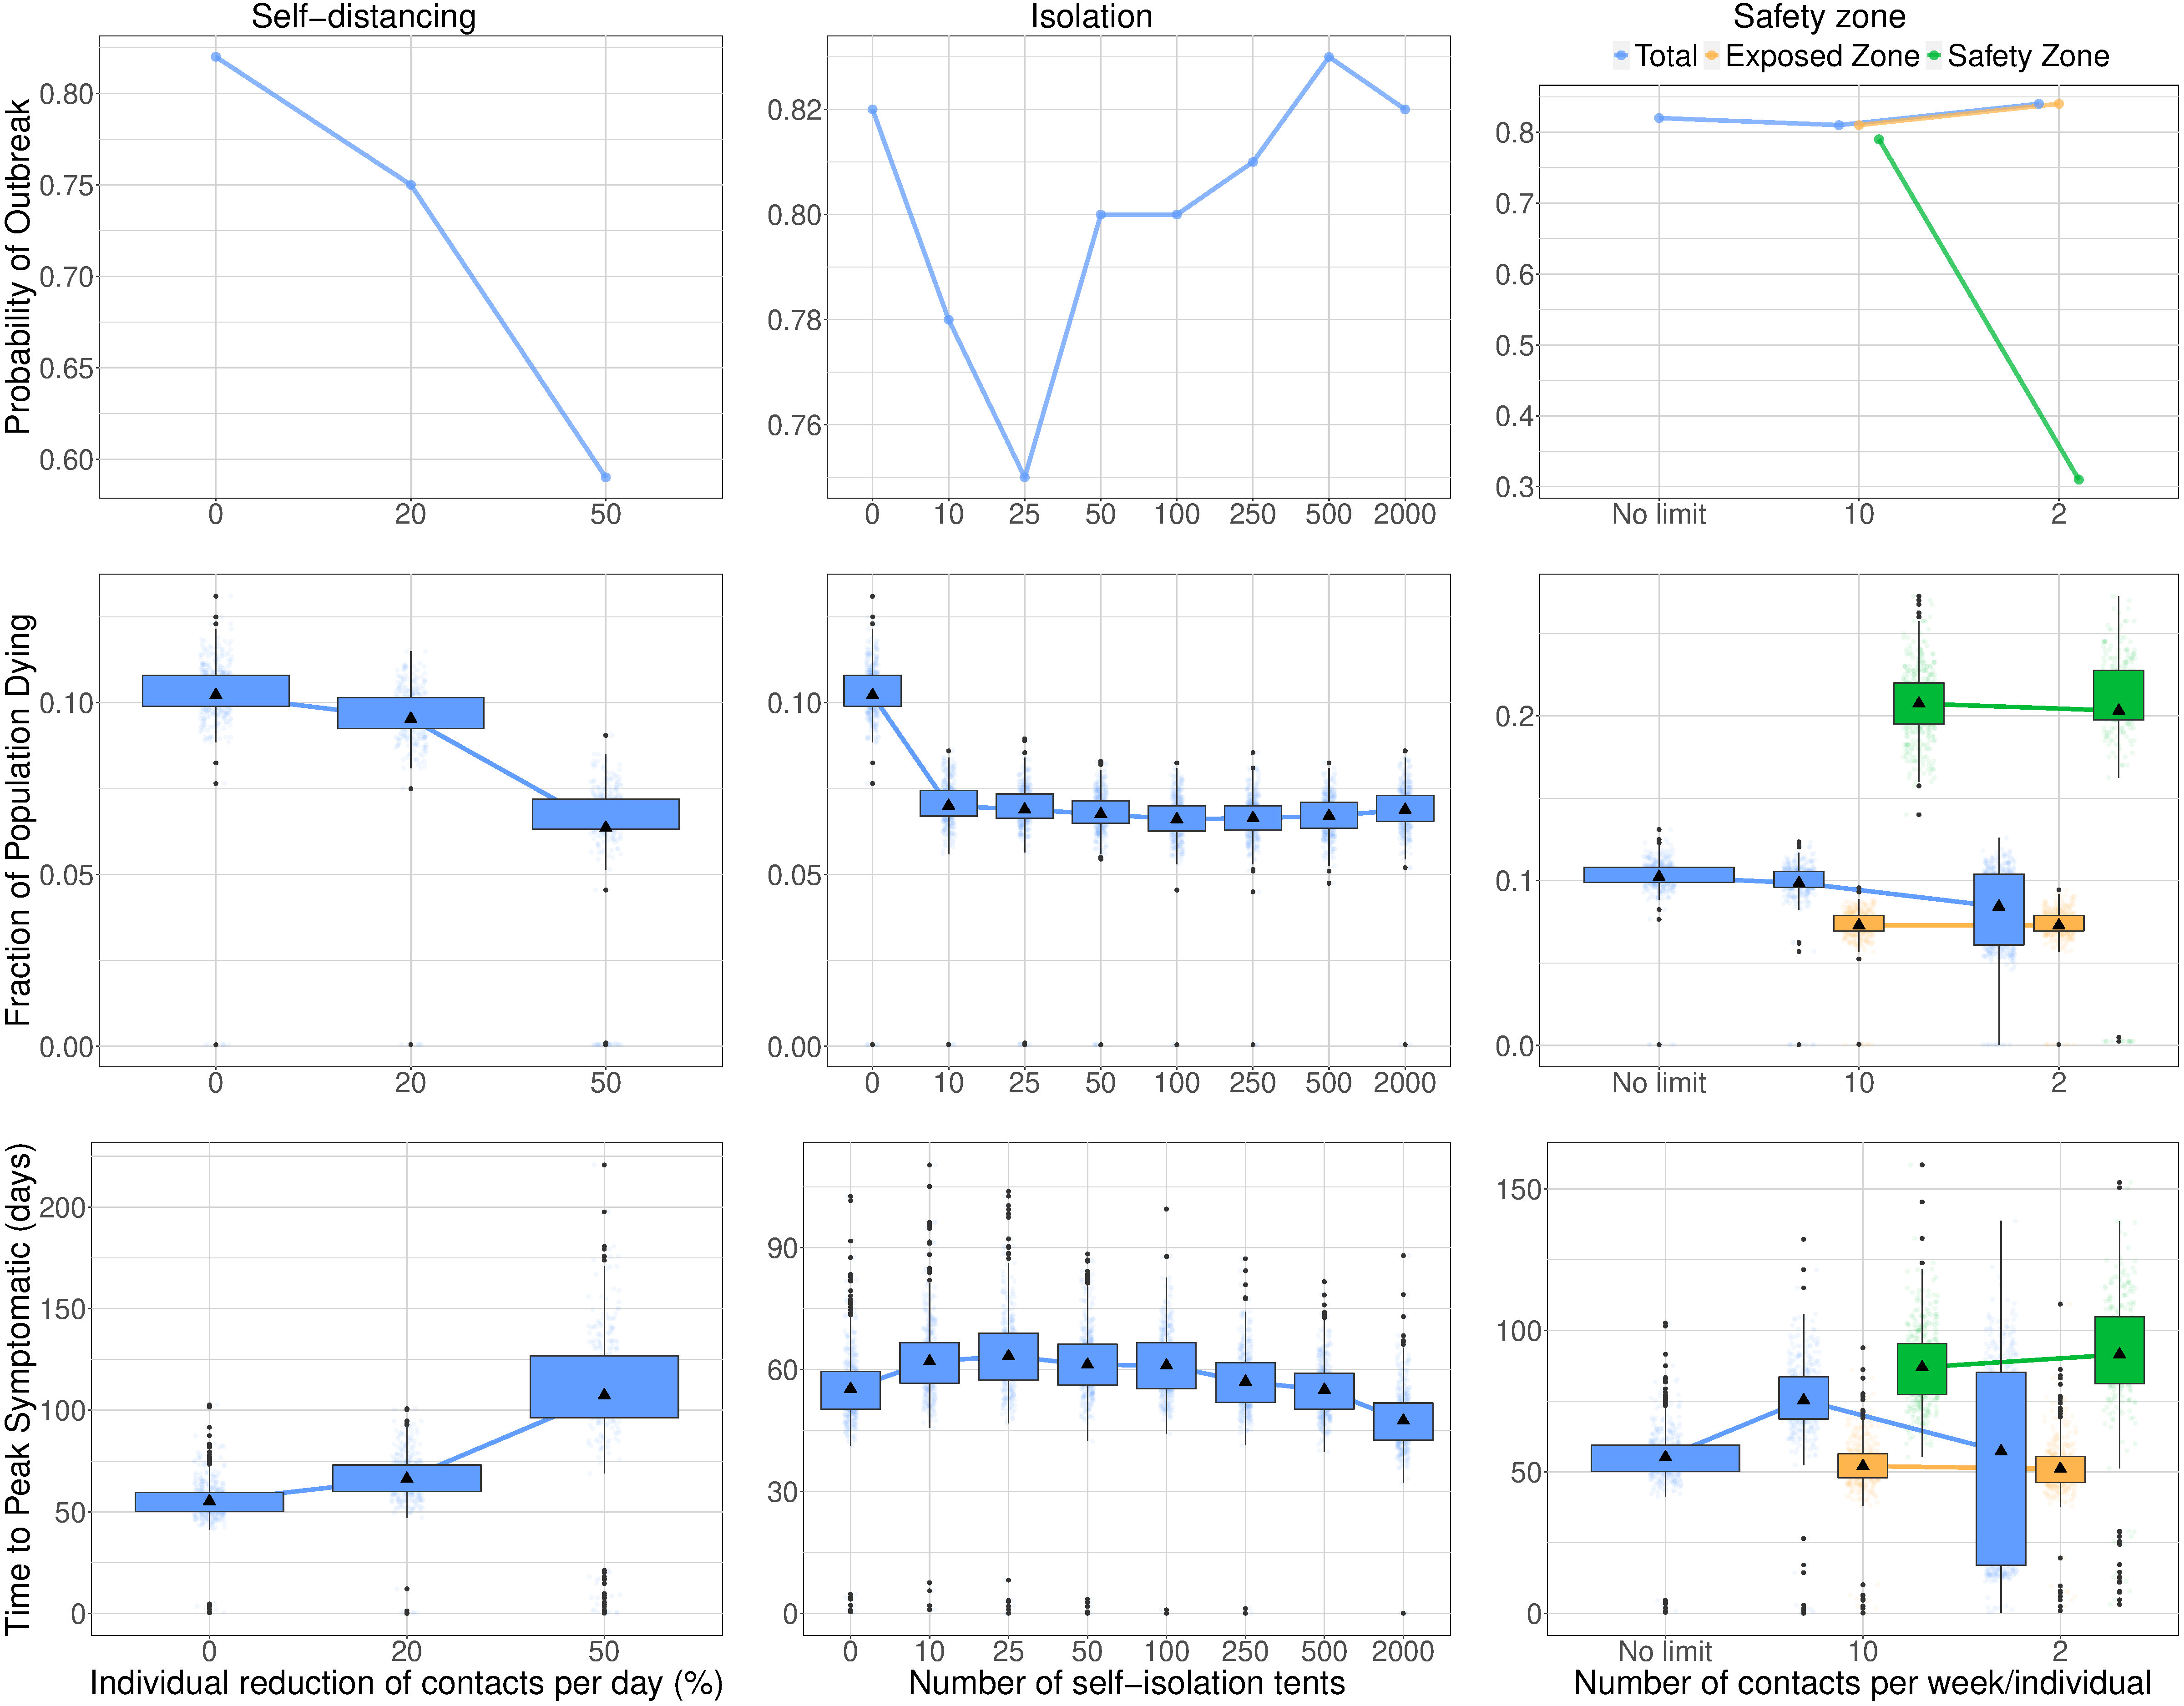
\includegraphics[width=1\textwidth]{figures/newFig/Fig2}

\caption{\label{fig:Panel2} \textbf{Effect of interventions on outbreak probability,
fatalities and time until synptomatic cases peak.} A: Self-distancing,
probability of an outbreak. B: Self-distancing, fraction of the population
dying. C: Self-distancing, time until peak symptomatic cases. D: Self-isolation,
probability of an outbreak. E: Self-isolation, fraction of the population
dying. F: Self-isolation, time until peak symptomatic cases. G: Safety
zone, probability of an outbreak. H: Safety zone, fraction of the
population dying. I: Safety zone, time until peak symptomatic cases.
Note that, for the safety zone, the mean of the whole is not the mean
of the exposed and safety zones, since means are computed considering
simulations in which at least one death was observed in the population
classes inhabitating the zone. This fact explains why in panel I there
is a reduction in the mean time for the whole population despite of
being a strong increase in the safety zone: in \textasciitilde 35\%
of the simulations there is an outbreak in the orange zone but not
in the green zone (panel G).}
\end{figure}

Self-distancing has a notable effect on reducing the probability of
an outbreak; even a 20\% reduction in daily contacts is associated
with a \textasciitilde 10\% decrease in outbreak probability (see
Fig. \ref{fig:Panel2}A). A greater reduction in daily contacts, of
50\%, is required to observe a significant decrease, of as much as
35\%, in the fraction of the population dying (see Fig. \ref{fig:Panel2}B).
A reduction in contacts of this magnitude also significantly extends
the time until the number of symptomatic cases peaks to 110 days,
roughly double the time when no interventions are in place (see Fig.
\ref{fig:Panel2}C). However, the proportion of the population recovered
after 12 months is reduced by \textasciitilde 30\% (see Supplementary
Fig. \ref{fig:Suppl_self})

With only 10 tents for a camp of 2000 people (i.e. 1 tent for every
200 people), self-isolation yields a modest decrease in the probability
of observing an outbreak (see Fig. \ref{fig:Panel2}D), but a stronger
reduction in mortality (\textasciitilde 30\%) (see Fig. \ref{fig:Panel2}E).
However, further increasing the number of tents significantly augment
this reduction up to 1 per every 10 people (Kruskal-Conover posthoc-test,
p-val$<3\times10^{-5}$) and, above this number, mortality even begin
to slightly increase again. This effect is a consequence of having
one carer per individual isolated (see Supplementary Material), so
when the isolated (infected) population increases, the number of healthy
working-age adults in contact with them increases in tandem. Nevertheless,
we observe a continuous reduction in CFR, albeit small, with an increasing
number of tents (see Supplementary Fig. \ref{fig:Suppl_isolation}).

Importantly, the potential reductions in overall fatalities and CFR
from self-isolation are realized whether the time required for individuals
to recognize their symptoms is 12h or 24h on average, but the intervention
becomes less effective when this time increases to 48h (see Supplementary
Fig. \ref{fig:Suppl_onset}). We observe no significant effects when
severe cases requiring hospitalization are evacuated (see Supplementary
Fig. \ref{fig:Suppl_evacuation}). Since we assume that evacuation
does not change their fate, this intervention only affects their infectivity.
Although the period between developing more severe symptoms and dying
is relatively long (\textasciitilde 10 days), the number of individuals
under these conditions is only a small fraction of the total infectious
population at any given time.

Creating a green zone improves the effect of previous interventions
overall, but with sometimes opposite outcomes for the exposed and
protected populations. For example, the probability of an outbreak
sharply decreases for the protected population, by almost 60\%, if
only two contacts are allowed per week in the buffer zone (see Fig.
\ref{fig:Panel2}G). Notably, most of this reduction is only achieved
when health-checks excluding symptomatic individuals from the buffer
zone are in place (see Supplementary Fig. \ref{fig:Suppl_Tcheck}).
On the other hand, the probability of an outbreak may slightly increase
for the exposed population, a consequence of the relative increase
in intra-zone contacts. Despite this side-effect, by shifting the
burden of an outbreak towards the less vulnerable population in the
orange zone, this intervention not only reduces fatalities among the
more vulnerable population in the green zone (Kruskal-Wallis test,
p-val$<10^{-15}$; see Supplementary Fig. \ref{fig:Suppl_agegroups}),
but also reduces the overall CFR (see Supplementary Fig. \ref{fig:Suppl_safety})
and thus the number of fatalities globally (see Fig. \ref{fig:Panel2}H).
Another important outcome of this intervention is the notable increase
in time until the number of symptomatic cases peaks for the vulnerable
population., This effect  is notobserved globally, when there is an
outbreak in the orange zone but not in the green zone (see Fig. \ref{fig:Panel2}I).

Considering different scenarios for allocating people to the green
zone, the lowest probability of an outbreak is achieved when only
older adults or at most older adults and working-age adults with comorbidities
move there (see Supplementary Fig. \ref{fig:Suppl_popClass}). Positive
effects of the green zone intervention are even more marked in camps
with smaller populations, for every outcome of interest except time
until symptomatic cases peak (see Supplementary Fig. \ref{fig:Suppl_popSize}).
The incorporation of a lockdown has the greatest effect on reducing
the probability of an outbreak in the green zone, to under 0.10. While
lockdowns show no positive effect on green zone fatalities in the
few instances where an outbreak does reach there, they decrease CFR
and overall fatalities by further concentrating outbreaks in the less
vulnerable population (see Supplementary Fig. \ref{fig:Suppl_lockdown}).

The effects of the interventions observed when we examine them individually
build upon each other when multiple interventions are implemented
in tandem (see Fig. \ref{fig:Panel3} and Supplementary Fig. \ref{fig:Suppl_combined}).
The protective effects of the safety zone intervention especially
are most fully realized when paired with other interventions, less
so when implemented on its own. When all interventions are implemented
together: strict self-distancing (50\% reduction in contacts), self-isolation
of symptomatic cases (1 tent for every 40 people), a safety zone with
2 contacts per week in the buffer zone, health checks and a moderate
lockdown (50\%), and evacuation of severe cases, mortality is reduced
by \textasciitilde 80\%.

\begin{figure}[H]
\begin{centering}
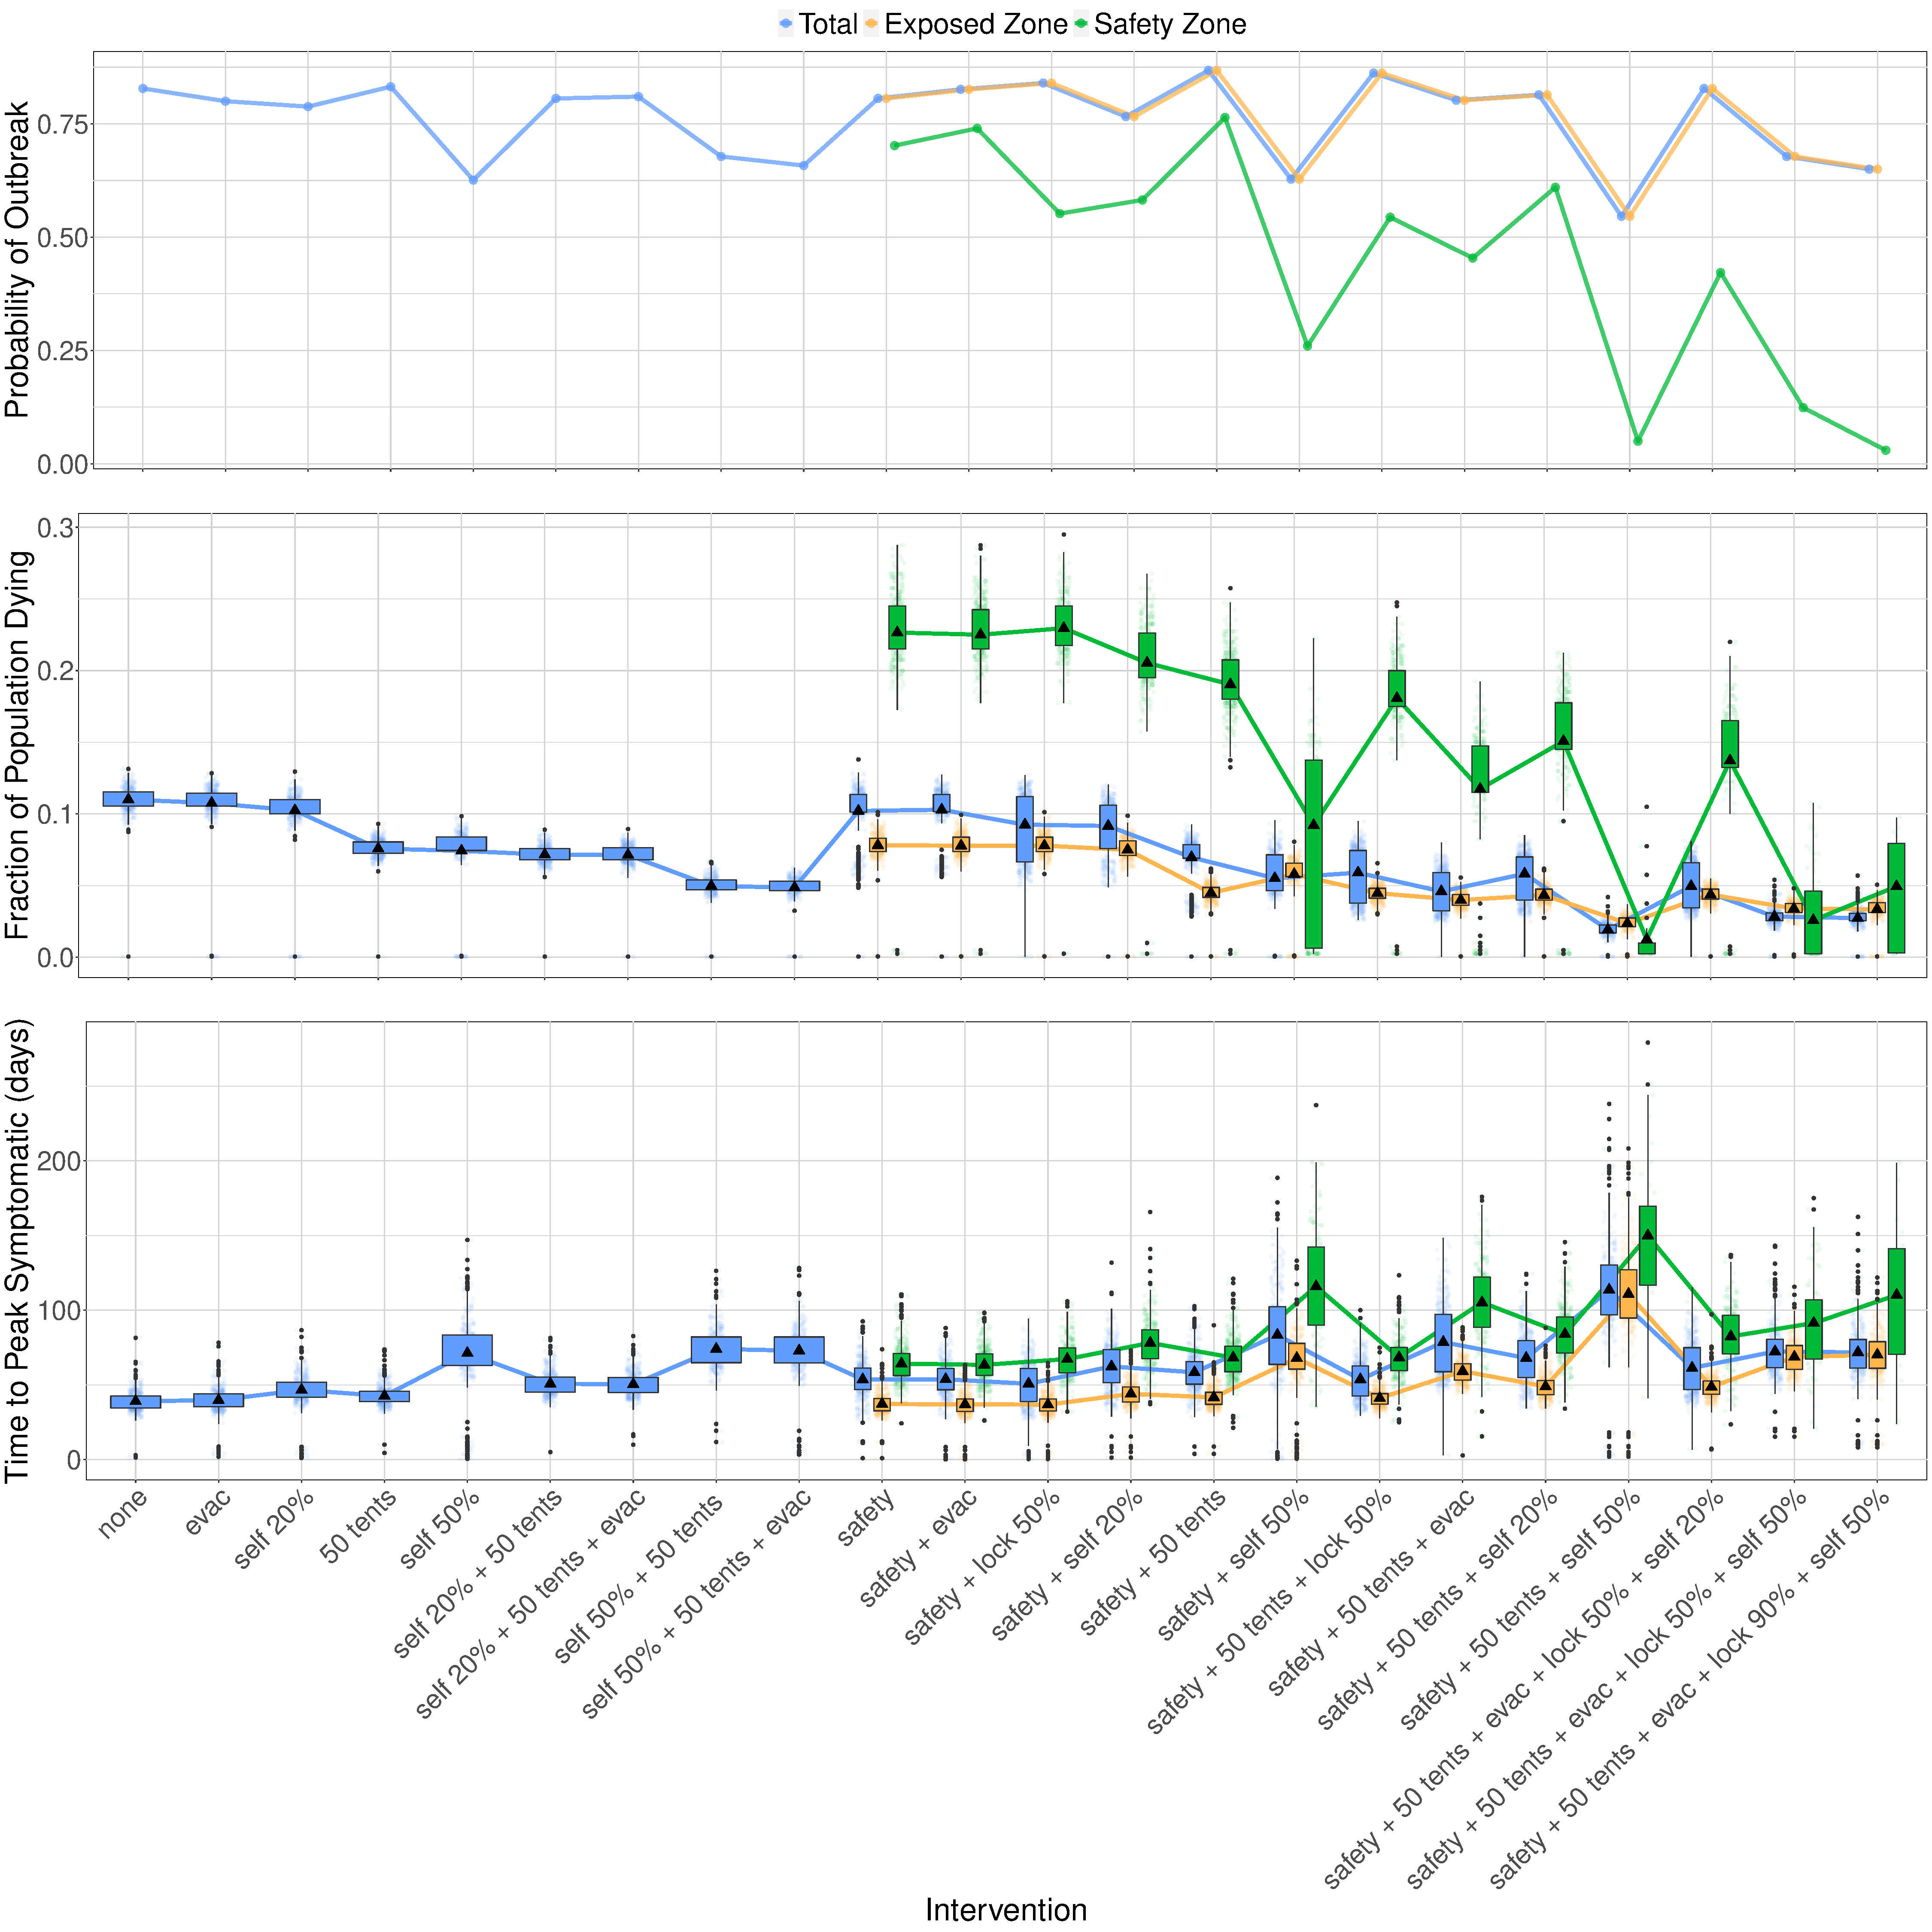
\includegraphics[width=1\textwidth]{figures/newFig/Fig3}\\
\par\end{centering}
\caption{\label{fig:Panel3} \textbf{Combinations of interventions.} Probability
of an outbreak (top), fraction of the population dying (middle) and
time until peak symptomatic cases (bottom) for different combination
of interventions. Evac = evacuation of severely symptomatic, self
= self-distancing, tents = number of available self-isolation tents,
safety = safety zone, lock = lockdown of the buffer zone. For combinations
of interventions including a safety zone, we distinguish between the
population living in the green zone, in the orange zone and the whole
population.}
\end{figure}


\part*{Discussion}

In this study, we propose a number of interventions of immediate applicability
to informal settlements. We focused on IDP settlements in NW Syria,
taking into account the interventions' feasibility, cultural acceptance
and their need for low-cost. When confronted with different possible
scenarios, we generally considered the worst-cases, highlighting the
interventions that are most effective in the direst conditions, but
possibly resulting in an overestimate of mortality. Our results align
with previous simulation studies of potential COVID-19 interventions
in similarly densely populated, low resource settings where informal
settlements are present, such as urban areas of sub-Saharan Africa.
In these settings, social-distancing is demonstrated to be an effective
intervention, and even small changes are estimated to have large effects
on outbreaks \cite{nyabadza2020}, in some cases determining whether
or not already inadequate healthcare systems become overwhelmed \cite{siraj_early_2020}.
Zandvoort et al. show that similar measures to the ones we consider:
self-isolation, physical distancing and ``shielding'' the vulnerable,
may reduce mortality by 60\%-75\% in African cities \cite{vanzandvoort2020}.

Self-distancing proves to be an effective measure in our models as
well; reducing contacts by 50\% has the greatest effect across the
most outcomes of interest of any of the interventions we examined.
However, the difficulty of achieving a reduction of this magnitude
cannot be overlooked, especially considering the large proportion
of the population composed of children, a group with an already high
contact rate that may prove difficult to control \cite{noauthor_syrian_nodate}.

We also propose self-isolation using individual tents which can be
located in a dedicated zone or next to the tents of relatives, where
contact with non-isolated individuals is mediated by a buffer zone.
This intervention is effective with even a small number of isolation
tents, as low as 5-10 tents per 1000 camp residents. After conversations
with camp managers, we found that this intervention is more likely
to be accepted in NW Syria than evacuation to community-based isolation
centers. Community-based isolation not only poses cultural challenges;
the capacity required to implement it has hardly been met \cite{UNOCHA_CCTC_numbers}.

One of the key parameters we assessed for the implementation of self-isolation
is the need for carers. In considering one carer per isolated individual,
with daily contact in a buffer zone, once a certain threshold of isolated
cases (\textasciitilde 200 per camp of 2000) is surpassed, the benefits
of isolation begin to be outweighed by an increase in infectivity
resulting from a growing number of exposed carers. This pitfall could
be circumvented through the creation of a more organized group of
carers, thus reducing the number of healthy working-age adults in
contact with isolated (infectious) individuals.

Much of the success or failure of the safety zone intervention hinges
on the functioning of the buffer zone. The number of inter-zone contacts
per week, the implementation of health checks, and potential lockdowns
all have notable effects. Also important is the portion of the population
that is protected; protecting only the vulnerable may have the most
beneficial effects, but it is precisely these vulnerable individuals,
older adults and people with comorbidities, who may most need family
members to care for them. While safety zone scenarios that allow greater
numbers of family members to accompany their vulnerable relatives
to the green zone may confer greater epidemiological risk, they may
also engender greater well-being and social cohesion.

Although setting up a safety zone sharply reduces the probability
of an outbreak in the population classes with the highest CFRs, thus
reducing the CFR of the entire population, it is possible that our
model may overestimate mortality from an outbreak in the green zone
in the few instances when there is one. Since total numbers of contacts
are conserved in our modelization, individuals do not reduce their
contacts when moved to the green zone, which implies an increase in
the number of contacts among vulnerable individuals. Despite of this
increase, we observed a significant reduction in the casualties in
the vulnerable population, when the safety zone is implemented. This
result answers concerns raised around this type of intervention due
to the large number of casualties registered in nursing-homes in wealthy
countries \cite{dahab_covidIDPcontrol_2020}. While in wealthy countries
individuals in a nursing-home will increase their exposure with respect
to living confined in their household, in the camps individuals moving
to the green zone will become less exposed. %
\begin{comment}
Our results show that there is a benefit even if there is no reduction
in the number of contacts. Since most of the camps in Idlib have no
management all these assumptions are unnecessary.
\end{comment}
{} 

An instrumental consideration for our models is the fraction of the
population recovered from COVID-19 after a steady state is reached.
Although the duration for which SARS-CoV-2 infection confers immunity
is uncertain, the proportion of the population recovered after an
outbreak should play a role in its protection against future ones.
For every intervention except self-distancing of 50\%, we observed
that the fraction of the population recovered meets or exceeds 75\%.
This is quite promising to prevent future outbreaks.

Unaccounted for social and cultural dynamics will undeniably complicate
the feasibility of our proposed interventions. One example we have
not addressed here is the unlikeliness of children under 13 self-isolating.
Although the number of of exceptions to the cases proposed are possibly
endless, the community-based nature of our approach may contribute
to circumvent these challenges much faster than health-based interventions,
which often depend on complex political decisions and may take years
to reach the needed level of response. If the dynamics of the virus
are well understood by local communities and at least some of the
interventions we propose are implemented, the impacts of COVID-19
can be mitigated even in an environment as challenging as NW Syria.

Given a rapidly changing environment and slow responses of local and
international authorities, empowering local communities themselves
is perhaps the best, if not the only way, to help them avoid the worst
consequences of the pandemic. This not only applies to IDP camps in
NW Syria, but to conflict-torn regions, informal settlements and vulnerable
communities around the world: from the urban slums of India, townships
of South Africa and favelas of Brazil, to the refugee camps of Kenya,
Bangladesh and South Sudan; the low-cost, effective interventions
we present are feasible, needed and urgent.

\subsection*{Acknowledgements}

This collaboration was organized by crowdfightCOVID19 (www.crowdfightcovid19.org)
upon request from CS. We thank Judith Boumann for valuable contributions.
We thank Peter Ashcroft, Juan Poyatos and members of Sebastian Bonhoeffer's
and Bryan Grenfell's groups for useful discussions. ECF research is
supported by Wellcome Trust grant 204833/Z/16/Z.

\subsection*{Conflicts of interests}

APG is a Board Member of crowdfightCOVID19, an initiative from the
scientific community to put all available resources at the service
of the fight against COVID-19. CS is a Board Member of the Pax Syriana
Foundation, a non-profit organization set up for social and philanthropic
purposes including promoting and providing support and assistance
to civilian aid projects in the fields of education, health, emergency
assistance, psychological assistance and humanitarian aid for people
affected by wars or humanitarian crisis. These organizations had no
role in study design, data collection, data analysis, data interpretation,
or writing of the article.

\bibliographystyle{unsrt}
\bibliography{req550-syria}

\end{document}
